\documentclass[thesis]{subfiles}

\begin{document}

\chapter{Testy}

Niniejszy rozdział opisuje przeprowadzone testy części \hyperref[sec:srv-app]{serwerowej} i~\hyperref[sec:cli-app]{klienckiej} aplikacji. Testy te~obejmują kilkukrotny cykl naprzemiennego dokonywania zmian w~elementach konfiguracji systemu wzorcowego, skanowania jego śledzonego drzewa plików, generowania \hyperref[sec:obraz-zmian-konfiguracji]{obrazu zmian konfiguracji systemu wzorcowego} za~pomocą aplikacji serwera \hyperref[sec:srv-app]{\texttt{\srvappname{}}} i~zastosowania go~na~systemie klienckim za~pomocą \hyperref[sec:cli-app]{aplikacji klienckiej \texttt{\cliappname{}}}. Cały cykl jest poprzedzony wstępnym skanowaniem systemu wzorcowego.

%------------------------------------------------------------------------------

\section{Podział testów}

Przeprowadzono dwa zasadnicze rodzaje testów funkcjonalnych aplikacji \hyperref[sec:cli-app]{klienckiej \texttt{\cliappname{}}} i~\hyperref[sec:srv-app]{aplikacji serwera \texttt{\srvappname{}}}:\mynobreakpar
\begin{enumerate}
	\item ,,małe'' --- doraźne, testujące obie aplikacje na~niewielkim drzewie katalogów opisanym w~załączniku~\ref{ch:aide-example} i~zobrazowanym na~rysunku~\ref{fig:drzewo-katalogow-przyklad-aide} (patrz listingi~\ref{lst:tree-create-aide-example} i~\ref{lst:tree-change-aide-example}) --- ten rodzaj testów jest częściowo zautomatyzowany przygotowanym w~ramach tej~pracy skryptem \path{dirtree-generator.sh}\footnote{Pomoc dotycząca sposobu użycia tego skryptu można uzyskać wywołując skrypt z~flagą \texttt{--help} lub~\texttt{-h}.}, który generuje przykładowe drzewo katalogów, a~następnie je modyfikuje w~sposób przedstawiony na~listingu~\ref{lst:tree-change-aide-example} w~załączniku~\ref{ch:aide-example}; testy przeprowadzone za~pomocą tego skryptu i~ich ręczne modyfikacje były pomocne do~względnie szybkiego testowania nowych funkcjonalności podczas implementowania projektu,
	\item ,,duże'' --- ręczne, tzn.~niezautomatyzowane testy na~,,czystym'', tzn.~dopiero~co zainstalowanym systemie operacyjnym \glslink{gnulinux}{Linux} \arch{} i~\debian{} --- testy te~obejmowały: skanowanie niemal całego systemu operacyjnego za~pomocą opcji \hyperlinktt{itm:srv-scan}{--scan} \hyperref[sec:srv-app]{aplikacji serwera} (z~wyłączeniem m.in.~katalogów wymienionych w~rozdziale~\ref{sec:aide}), ręczne modyfikowanie jego wybranych elementów konfiguracji, generowanie \hyperref[sec:obraz-zmian-konfiguracji]{obrazu zmian konfiguracji systemu wzorcowego}, udostępnienie go~klientom i~zastosowanie go~przez nich; ze~względu na~swój kompleksowy, całościowy charakter, pracochłonność i~trudność ich zautomatyzowania, pochłonęły znacznie więcej czasu niż doraźne testy i~dlatego były kilkukrotnie przeprowadzone tylko pod~koniec projektu.
\end{enumerate}

,,Małe testy'' zostały przeprowadzone na~jednym komputerze stacjonarnym. Wszystkie ,,duże testy'' wykonano w~środowisku złożonym z~trzech fizycznych komputerów \href{https://en.wikipedia.org/wiki/Personal_computer}{klasy~PC}. Schemat ich~konfiguracji sieciowej został przedstawiony na~rysunku~\ref{fig:testing-network}. Każdy z~komputerów testowych miał zainstalowany systemem operacyjny \linuxdebian{} oraz~maszynę wirtualną \hrefemph{https://www.virtualbox.org/}{VirtualBox~5.1} z~zainstalowanym na~niej ,,czystym'', tzn.~dopiero co~zainstalowanym systemem operacyjnym \linuxarch{}. Testy ,,duże'' zostały przeprowadzone w~dwóch wariantach, aby~sprawdzić zarówno obsługę dystrybucji \linuxarch{}, jak i~\linuxdebian{} --- w~pierwszym z~nich wszystkie testowane komputery działały na~wirtualizowanym systemie \arch{}, a~w~drugim na~natywnie zainstalowanym systemie \debian{}\footnote{Zgodnie z~uwagami dotyczącymi obsługiwanych dystrybucji \glslink{gnulinux}{Linux} zamieszczonymi na~końcu rozdziału~\ref{sec:obraz-zmian-konfiguracji}.}. W~każdym z~tych wariantów jeden z~komputerów odgrywał rolę stacji wzorcowej, a~pozostałe klientów.

\begin{figure}
	\centering
	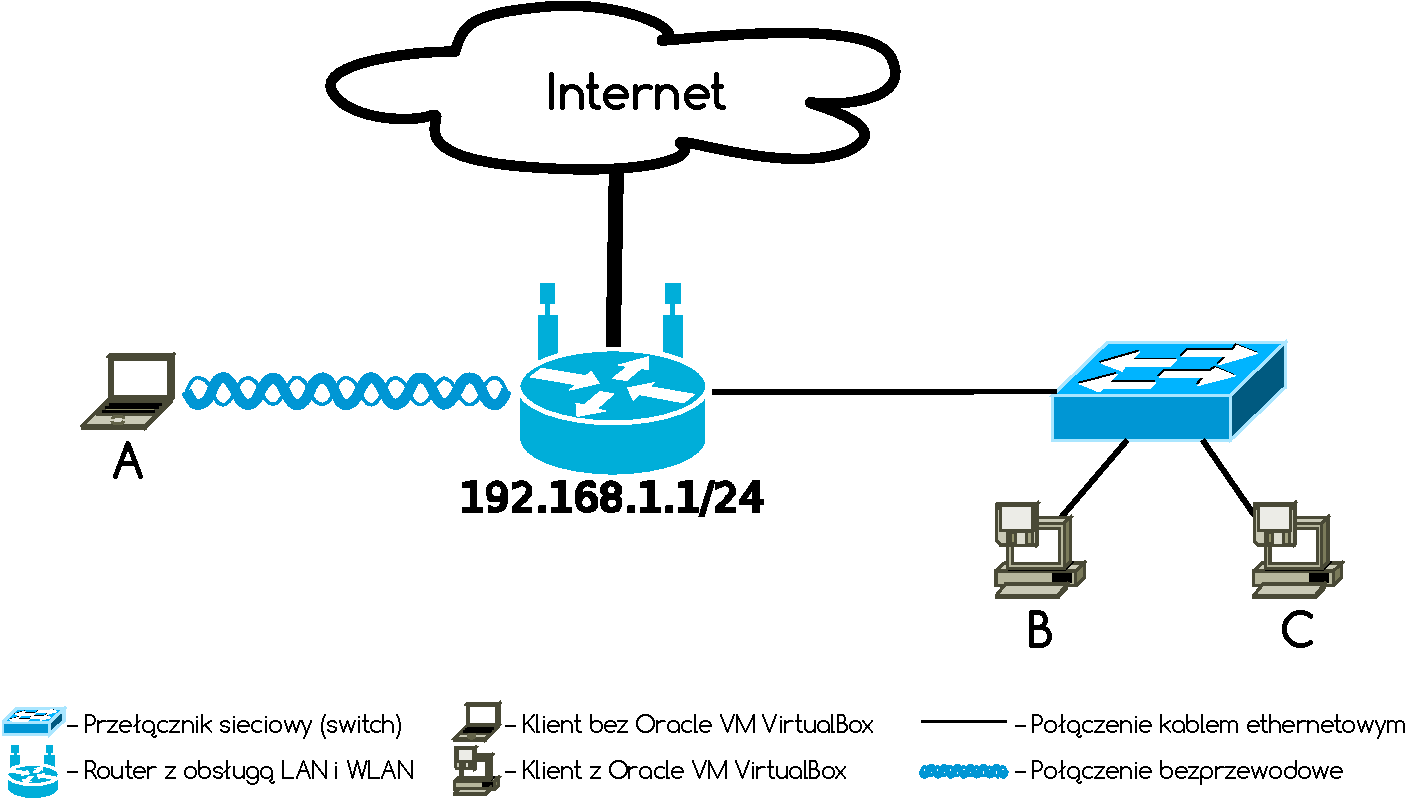
\includegraphics[width=0.46\textwidth]{img/testing-network}
	\caption{Schemat przedstawiający konfigurację sieciową użytego środowiska testowego}
	\label{fig:testing-network}
\end{figure}

W~kolejnych dwóch rozdziałach~\ref{sec:male-testy} i~\ref{sec:duze-testy} zostały przybliżone oba rodzaje przeprowadzonych testów, tzn.~tych umownie nazwanych ,,małymi'' i~,,dużymi''.

%------------------------------------------------------------------------------

\section{Małe testy}
\label{sec:male-testy}

% Listingi~\ref{lst:male-testy-pierwsze-skanowanie}, \ref{lst:male-testy-utworzenie-drzewa}, \ref{lst:male-testy-drugie-skanowanie}, \ref{lst:male-testy-generowanie-obrazu-0}, \ref{lst:male-testy-zmiany-w-drzewie}, \ref{lst:male-testy-trzecie-skanowanie}, \ref{lst:male-testy-generowanie-obrazu-1}, \ref{lst:zastosowanie-obrazu-0} i~\ref{lst:zastosowanie-obrazu-1} (...)
Przeprowadzenie ,,małych testów'' jest względnie proste, ponieważ w~przeciwieństwie do~testów ,,dużych'' są~one częściowo zautomatyzowane i~nie wymagają dużo czasu do~skonfigurowania. Listingi~\ref{lst:male-testy-pierwsze-skanowanie}--\ref{lst:zastosowanie-obrazu-1} przedstawiają 9~kolejnych kroków testowania aplikacji serwera i~klienta na~przykładowym drzewie plików opisanym w~rozdziale~\ref{sec:aide} i~zobrazowanym na~rysunku~\ref{fig:drzewo-katalogow-przyklad-aide} wg scenariusza ,,małych testów''. Użyty na~podanych listingach w~wywołaniach aplikacji \texttt{\srvappname{}} parametr \path{/tmp/myscm_aide_test.conf} dla~opcji \hyperlink{itm:aide-config}{\texttt{--aide-config}} to~ścieżka do~pliku konfiguracyjnego przygotowanego na~potrzeby ,,małego testu'' --- jego zawartość została przedstawiona na~listingu~\ref{lst:male-testy-plik-konfiguracyjny} na~stronach~\pageref{lst:male-testy-plik-konfiguracyjny}--\pageref{male-testy-plik-konfiguracyjny-last-page} wraz z~komentarzami\footnote{Komentarze z~sekcji \hyperref[line:aide-syntax-section]{\texttt{AIDE SYNTAX SECTION}} konfiguracji \path{myscm_aide_test.conf} z~listingu~\ref{lst:male-testy-plik-konfiguracyjny} są~zapożyczone z~\glslink{manual}{manuala} \hreftt{https://www.systutorials.com/docs/linux/man/5-aide.conf/}{aide.conf(5)} dostarczonego przez \href{https://packages.debian.org/search?keywords=aide}{Debianowy} pakiet oprogramowania \hyperref[sec:aide]{AIDE}.}, aby~ułatwić Czytelnikowi zrozumienie jakie jest znaczenie poszczególnych zmiennych konfiguracyjnych dla~działania aplikacji.

Listing~\ref{lst:male-testy-pierwsze-skanowanie} demonstruje pierwsze skanowanie części systemu zdefiniowanej w~pliku konfiguracyjnym \path{myscm_aide_test.conf} z~listingu~\ref{lst:male-testy-plik-konfiguracyjny}. Wśród komunikatów jakie pojawiły się po~rozpoczęciu skanowania dają się zauważyć ostrzeżenia (\texttt{WARNING}i), które informują o~tym, że~w~normalnym trybie użytkowania aplikacji powinna ona być uruchamiana z~prawami administratora, aby~móc skanować elementy systemu dostępne tylko dla~użytkownika \superuser{} oraz~o~tym, że~w~skanowanym drzewie nie znaleziono 3~plików i~1~katalogu wymienionych w~konfiguracji \path{myscm_aide_test.conf} z~listingu~\ref{lst:male-testy-plik-konfiguracyjny}. Ostrzeżenia te~można w~tym wypadku zignorować, ponieważ do~skanowania testowych katalogów nie są~potrzebne prawa administratora, a~brakujące pliki są~tworzone w~kolejnym kroku testów, przedstawionym na~listingu~\ref{lst:male-testy-utworzenie-drzewa}. W~przypadku chęci dokładniejszej analizy tego co~robi aplikacja \texttt{\srvappname{}} podczas swojego działania, można dodać do~jej wywołania flagę \hyperlinktt{itm:verbosity}{--verbose}, która dodaje do~wyświetlanych i~zapisywanych w~logach komunikatów nowy ich~rodzaj, tj.~\texttt{DEBUG}\footnote{Dla~zachowania czytelności listingów zrezygnowano z~wywołania \texttt{\srvappname{}} z~flagą \hyperlinktt{itm:verbosity}{--verbose}.}.

\begin{lstlisting}[language=,basicstyle=\fontsize{8}{9}\ttfamily,caption={Pierwsze skanowanie drzewa katalogów zdefiniowanego w~konfiguracji \protect\path{/tmp/myscm_aide_test.conf} za~pomocą aplikacji \texttt{\srvappname{}} \emph{przed} stworzeniem testowego drzewa katalogów za~pomocą skryptu \texttt{dirtree-generator.sh}},label=lst:male-testy-pierwsze-skanowanie]
user@host~$ ./myscm-srv.py --aide-config /tmp/myscm_aide_test.conf --scan
WARNING [2017-08-20 16:32:22,392] This application is supposed to be ran with root permissions. Root permissions may be not needed if you don't need to scan restricted parts of the filesystem.
INFO [2017-08-20 16:32:22,393] Running 'aide --check -c /tmp/myscm_aide_test.conf' command to check if aide.db is up-to-date. It may take some time to finish...
INFO [2017-08-20 16:32:22,436] Running 'aide --init -c /tmp/myscm_aide_test.conf' command to create new aide.db. It may take some time to finish...
WARNING [2017-08-20 16:32:22,446] File '/tmp/demo/dir3_symlink/file8' specified in '/tmp/myscm_aide_test.conf' (line 121) doesn't exist - skipping.
WARNING [2017-08-20 16:32:22,447] File '/tmp/demo/file1' specified in '/tmp/myscm_aide_test.conf' (line 122) doesn't exist - skipping.
WARNING [2017-08-20 16:32:22,447] File '/tmp/demo/dir3/file8' specified in '/tmp/myscm_aide_test.conf' (line 123) doesn't exist - skipping.
WARNING [2017-08-20 16:32:22,448] File '/tmp/demo/dir3' specified in '/tmp/myscm_aide_test.conf' (line 124) doesn't exist - skipping.
INFO [2017-08-20 16:32:22,448] New reference AIDE database '/tmp/aide.db.current/aide.db' setup successful. Run --list-db option to list all available AIDE databases created so far.
\end{lstlisting}

\begin{lstlisting}[language=,basicstyle=\fontsize{8}{9}\ttfamily,caption={Utworzenie testowego drzewa katalogów \protect\path{/tmp/demo} za~pomocą skryptu \protect\path{dirtree-generator.sh}},label=lst:male-testy-utworzenie-drzewa,numbers=none]
user@host:~$ ./dirtree-generator.sh /tmp/demo
\end{lstlisting}

Listing~\ref{lst:male-testy-drugie-skanowanie} przedstawia wywołanie drugiego skanowania, już po~stworzeniu testowego drzewa katalogów \path{/tmp/demo}, utworzonego za~pomocą wywołania skryptu \path{dirtree-generator.sh} z~listingu~\ref{lst:male-testy-utworzenie-drzewa}. Warto zauważyć, że~na~listingu~\ref{lst:male-testy-drugie-skanowanie} nie ma już ostrzeżeń widocznych na~listingu~\ref{lst:male-testy-pierwsze-skanowanie} dotyczących brakujących plików --- są~za~to komunikaty informujące m.in.~o~uruchomieniu \hyperref[sec:aide]{AIDE} z~flagą \texttt{--check}, a~następnie z~flagą \texttt{--init} (są~one również na~listingu~\ref{lst:male-testy-pierwsze-skanowanie}). Pierwsze z~tych wywołań sprawdza czy~w~systemie zaszły jakieś zmiany od~czasu ostatniego skanowania --- jeśli nie, to~tworzenie nowej bazy \hyperref[sec:aide]{AIDE} za~pomocą flagi \texttt{--init} byłoby niepotrzebne i~aplikacja zakończyłaby działanie z~komunikatem wyjaśniającym swoje wczesne zakończenie. Kolejne komunikaty informują o~tym, że~po~przeprowadzonym skanowaniu \hyperref[sec:aide]{AIDE} został utworzony katalog \path{/tmp/aide.db.current} z~informacjami o~stanie przeskanowanego systemu. W~skład tego katalogu wchodzi plik stanu \path{/tmp/aide.db.current/aide.db} stworzony przez \hyperref[sec:aide]{AIDE} podczas jego uruchomienia z~flagą \texttt{--init} oraz~katalog \texttt{COPIED} zawierający pliki tekstowe wymienione w~sekcji \hyperref[line:extended-aide-syntax-section]{\texttt{EXTENDED AIDE SYNTAX SECTION}} pliku konfiguracyjnego z~listingu~\ref{lst:male-testy-plik-konfiguracyjny}, która definiuje dla~których plików powinna być możliwość tworzenia \hrefemph{https://en.wikipedia.org/wiki/Patch_(Unix)}{patchy}, które znajdą się w~\hyperref[sec:obraz-zmian-konfiguracji]{obrazie konfiguracji systemu wzorcowego} generowanego za~pomocą opcji \hyperlinktt{itm:srv-gen-img}{--gen-img} aplikacji \hyperref[sec:srv-app]{serwera}. Pliki niewymienione w~tej sekcji są~kopiowane w~całości do~generowanego \hyperref[sec:obraz-zmian-konfiguracji]{obrazu zmian}. Oczywiście zarówno \hrefemph{https://en.wikipedia.org/wiki/Patch_(Unix)}{patche}, jak i~całe pliki są~kopiowane do~\hyperref[sec:obraz-zmian-konfiguracji]{obrazu zmian} warunkowo, tzn.~tylko wtedy, gdy~klient tego pliku nie~ma lub~ma jego starszą wersję. Jeśli klient ma~już aktualną wersję pliku, to~nie trafia on~do~\hyperref[sec:obraz-zmian-konfiguracji]{obrazu konfiguracji systemu wzorcowego}. \hyperref[sec:srv-app]{Aplikacja serwera} wie które pliki ma~klient z~argumentu opcji \hyperlinktt{itm:srv-gen-img}{--gen-img}, który jest liczbą naturalną odpowiadającą deklarowanemu stanowi konfiguracji systemu klienta. Na~podstawie tej liczby serwer wyszukuje pliku stanu opisującego stan klienta i~porównuje taki plik do~pliku opisującego aktualny stan serwera --- takie porównanie odbywa się za~pomocą uruchomienia \hyperref[sec:aide]{AIDE} z~flagą \texttt{--check} działającą na~tymczasowym pliku konfiguracyjnym wygenerowanym przez \texttt{myscm-srv} (widocznym na~listingu~\ref{lst:male-testy-generowanie-obrazu-0} pod~nazwą \path{/tmp/tmpphgh4nl6.aide.conf}\footnote{Tymczasowe pliki konfiguracyjne są~tworzone za~pomocą modułu \python{} \hreftt{https://docs.python.org/dev/library/tempfile.html}{tempfile} --- stąd ich (pseudo)losowe nazwy.}).

\begin{lstlisting}[language=,basicstyle=\fontsize{8}{9}\ttfamily,caption={Drugie skanowanie drzewa katalogów zdefiniowanego w~konfiguracji \protect\path{/tmp/myscm_aide_test.conf} za~pomocą aplikacji \texttt{\srvappname{}} \emph{po}~stworzeniu testowego drzewa katalogów za~pomocą skryptu \texttt{dirtree-generator.sh}},label=lst:male-testy-drugie-skanowanie,escapechar=?]
user@host:~$ ./myscm-srv.py --aide-config /tmp/myscm_aide_test.conf --scan
WARNING [2017-08-20 16:44:29,605] This application is supposed to be ran with root permissions. Root permissions may be not needed if you don't need to scan restricted parts of the filesystem.
INFO [2017-08-20 16:44:29,606] Running 'aide --check -c /tmp/myscm_aide_test.conf' command to check if aide.db is up-to-date. It may take some time to finish...
INFO [2017-08-20 16:44:29,611] Running 'aide --init -c /tmp/myscm_aide_test.conf' command to create new aide.db. It may take some time to finish...
INFO [2017-08-20 16:44:29,619] Copying 4 files and/or directories selected in AIDE configuration '/tmp/myscm_aide_test.conf' to '/tmp/aide.db.current/COPIED' directory. Please wait, it may take some time to finish...
INFO [2017-08-20 16:44:29,620] New reference AIDE database '/tmp/aide.db.current/aide.db' setup successful. Run --list-db option to list all available AIDE databases created so far?\label{line:list-db-option}?
\end{lstlisting}

Listę wszystkich katalogów stanów utworzonych do~tej pory za~pomocą uruchomienia aplikacji \hyperref[sec:srv-app]{serwera} z~flagą \hyperlinktt{itm:srv-scan}{--scan} można wyświetlić za~pomocą opcji \hyperlinktt{itm:list-db}{--list-db}, o~czym informuje komunikat w~linii~\ref{line:list-db-option} na~listingu~\ref{lst:male-testy-drugie-skanowanie}. Aplikacja \hyperref[sec:srv-app]{serwera} zna~kolejną liczbę, która zostanie użyta do~nazwania katalogu utworzonego za~pomocą flagi \hyperlinktt{itm:srv-scan}{--scan} dzięki zawartości pliku tesktowego zapisanego domyślnie w~pliku \path{/var/myscm-cli/img_ver.myscm-cli} --- plik ten zawiera liczbę dotychczasowych wywołań skanowań zakończonych utworzeniem kolejnego katalogu z~opisem aktualnego stanu systemu wzorcowego.

Po~przeskanowaniu systemu wzorcowego przed i~po~utworzeniu drzewa katalogów \path{/tmp/demo} można wygenerować pierwszy \hyperref[sec:obraz-zmian-konfiguracji]{obraz zmian konfiguracji systemu wzorcowego}, przeznaczony dla~klientów, których konfiguracja jest w~stanie oznaczonym liczbą \texttt{0}, chcących się aktualizować do~stanu \texttt{1}. Wygenerowanie takiego obrazu zostało przedstawione na~listingu~\ref{lst:male-testy-generowanie-obrazu-0} --- widać na~nim w~linii~\ref{line:files-added-info}, że~do~wygenerowanego \hyperref[sec:obraz-zmian-konfiguracji]{obrazu zmian} zostały dodane 23~pliki\footnote{Nie licząc \href{https://en.wikipedia.org/wiki/Hard_link}{dowiązań twardych}.}, 0~zostało oznaczonych jako usunięte i~zmienione.

\begin{minipage}{\linewidth}
\begin{lstlisting}[language=,basicstyle=\fontsize{8}{9}\ttfamily,caption={Wygenerowanie obrazu zmian konfiguracji systemu wzorcowego \protect\path{myscm-img.0.1.tar.gz} i~jego podpisu cyfrowego, przeznaczonego dla~klientów w~stanie~\texttt{0}, chcących zaktualizować konfigurację swojego systemu do~stanu~\texttt{1}},label=lst:male-testy-generowanie-obrazu-0,escapechar=?]
user@host:~$ ./myscm-srv.py --aide-config /tmp/myscm_aide_test.conf --gen-img 0
WARNING [2017-08-20 16:46:14,415] This application is supposed to be ran with root permissions. Root permissions may be not needed if you don't need to scan restricted parts of the filesystem.
INFO [2017-08-20 16:46:14,416] Running 'aide --check -c /tmp/myscm_aide_test.conf' command to check if aide.db is up-to-date. It may take some time to finish...
INFO [2017-08-20 16:46:14,423] Generating system image based on current server's configuration and AIDE database file '/tmp/aide.db.0/aide.db.0' corresponding to client's system configuration.
INFO [2017-08-20 16:46:14,426] Running 'aide --check -c /tmp/tmpphgh4nl6.aide.conf' command to check if aide.db is up-to-date. It may take some time to finish...
INFO [2017-08-20 16:46:14,439] 23 files added, 0 removed, 0 changes since client's declared last update.?\label{line:files-added-info}?
INFO [2017-08-20 16:46:14,476] Adding to the system image 23 new files that were added to the tracked directories...
100% (23 of 23) |###################################| Elapsed Time: 0:00:29 Time: 0:00:29?\label{line:progress-bar}?
INFO [2017-08-20 16:46:44,093] No files were removed from the tracked directories, thus list of files removed from the system is empty.
| 0 Elapsed Time: 0:00:00
INFO [2017-08-20 16:46:44,095] No files were changed within tracked directories, thus list of changed files that was added to the system image is empty.
| 0 Elapsed Time: 0:00:00
INFO [2017-08-20 16:46:44,097] Successfully created system image '/tmp/myscm-img.0.1.tar.gz' for client identified by AIDE's database '/tmp/aide.db.0/aide.db.0'.

Enter password protecting 'certificate.key' private key of the SSL
certificate to digitally sign system image 'myscm-img.0.1.tar.gz'. If you want
to skip generating SSL signature press CTRL+C (or send SIGINT signal in any
other way).

Password: minipw

INFO [2017-08-20 16:46:47,372] Signature of the system image '/tmp/myscm-img.0.1.tar.gz.sig' created successfully!
\end{lstlisting}
\end{minipage}

Warto zwrócić uwagę na~pasek postępu przedstawiony w~linii~\ref{line:progress-bar} listingu~\ref{lst:male-testy-generowanie-obrazu-0} --- po~jego prawej stronie jest wypisany czas jaki trwało dodanie plików do~generowanego obrazu. W~tym przypadku taka operacja zajęła aż~29~sekund tylko~dla~23~plików. Takiemu wynikowi jest winne użycie komendy \hreftt{http://man7.org/linux/man-pages/man1/dpkg-query.1.html}{dpkg-query~--search} (lub~\hreftt{https://wiki.debian.org/apt-file}{apt-file search} jeśli jest zainstalowany) na~systemie \debian{} i~\hreftt{https://www.archlinux.org/pacman/pacman.8.html}{pacman --query --owns} na~systemie~\arch{}. Komendy te~obsługują menadżery pakietów i~służą do~pobrania nazwy pakietu oprogramowania do~którego należy zadany plik. Pobranie nazwy pakietu pliku dodanego do~\hyperref[sec:obraz-zmian-konfiguracji]{obrazu zmian} ma~na~celu oznaczenie go~jako zainstalowanego lub~odinstalowanego po~stronie klienta. W~przedstawionym przykładzie żaden z~plików nie należy do~żadnego pakietu, ponieważ wszystkie zostały wygenerowane za~pomocą skryptu \texttt{dirtree-generator.sh}. Dla~żadnego z~dodanych 23~plików aplikacja nie znalazła za~pomocą \hreftt{http://man7.org/linux/man-pages/man1/dpkg-query.1.html}{dpkg-query~--search} żadnego pakietu do~którego zadany plik należy, dlatego uruchamiała komendę \hreftt{https://wiki.debian.org/apt-file}{apt-file search}\footnote{Przedstawione listingi testów zostały przygotowane na~systemie \debian{} z~zainstalowanym zarówno \hreftt{http://man7.org/linux/man-pages/man1/dpkg-query.1.html}{dpkg-query}, jak i~\hreftt{https://wiki.debian.org/apt-file}{apt-file} (który nie jest wymagany do~działania \texttt{\srvappname{}}).} (\hrefemph{https://en.wikipedia.org/wiki/Fallback}{fallback}) która również nie znajdywała żadnego pakietu, przez co~czas generowania \hyperref[sec:obraz-zmian-konfiguracji]{obrazu zmian} jest tak duży. W~typowym przypadku użycia \texttt{\srvappname{}} zazwyczaj dodawane pliki należą do~jakiegoś pakietu zainstalowanego z~repozytorium pakietów i~czas działania podanych komend dla~jednego pliku jest krótszy.

Kolejnym krokiem testów jest wywołanie skryptu \texttt{dirtree-generator.sh} z~flagą \texttt{-m} (skrót opcji od~\emph{modify}), która dokonuje zmian w~zadanym drzewie katalogów \path{/tmp/demo} przedstawionych na~listingu~\ref{lst:tree-change-aide-example} w~załączniku~\ref{ch:aide-example}~(por. listing~\ref{lst:male-testy-zmiany-w-drzewie}), a~następnie ponowne, trzecie skanowanie systemu przedstawione na~listingu~\ref{lst:male-testy-trzecie-skanowanie}. W~linii~\ref{line:copied-files} listingu~\ref{lst:male-testy-trzecie-skanowanie} znajduje się informacja o~tym, że~w~wyniku skanowania systemu wzorcowego do~katalogu \path{/tmp/aide.db.current/COPIED} zostały skopiowane 4~pliki --- te~4~pliki to~pliki wymienione w~sekcji \hyperref[line:extended-aide-syntax-section]{\texttt{EXTENDED AIDE SYNTAX SECTION}} w~liniach \ref{line:first-copied-file}--\ref{line:last-copied-file} pliku konfiguracyjnego \path{myscm_aide_test.conf} z~listingu~\ref{lst:male-testy-plik-konfiguracyjny}. Kopiowanie do~katalogu \path{COPIED} zostało zaimplementowane po~to, aby w~przypadku potrzeby wygenerowania \hyperref[sec:obraz-zmian-konfiguracji]{obrazu zmian systemu wzorcowego} aktualizującego klienta ze~stanu utworzonego na~skutek aktualnego skanowania do~nowszego stanu, w~którym któryś z~tych plików został zmodyfikowany, można było dla~takiego pliku stworzyć \hrefemph{https://en.wikipedia.org/wiki/Patch_(Unix)}{patch} zamiast kopiować go~w~całości do~wynikowego \hyperref[sec:obraz-zmian-konfiguracji]{obrazu zmian}.

\begin{lstlisting}[language=,basicstyle=\fontsize{8}{9}\ttfamily,caption={Dokonanie przykładowych zmian w~drzewie katalogów \protect\path{/tmp/demo} przedstawionych na~listingu~\ref{lst:tree-change-aide-example} w~załączniku~\ref{ch:aide-example} za~pomocą skryptu \texttt{dirtree-generator.sh}},label=lst:male-testy-zmiany-w-drzewie,numbers=none]
user@host:~$ ./dirtree-generator.sh -m /tmp/demo
\end{lstlisting}

\begin{minipage}{\linewidth}
\begin{lstlisting}[language=,basicstyle=\fontsize{8}{9}\ttfamily,caption={Trzecie skanowanie drzewa katalogów zdefiniowanego w~konfiguracji \protect\path{/tmp/myscm_aide_test.conf} za~pomocą aplikacji \texttt{\srvappname{}} po~stworzeniu testowego drzewa katalogów i~dokonaniu na~nim zmian za~pomocą skryptu \texttt{dirtree-generator.sh}},label=lst:male-testy-trzecie-skanowanie,escapechar=?]
user@host:~$ ./myscm-srv.py --aide-config /tmp/myscm_aide_test.conf --scan
WARNING [2017-08-20 16:47:52,589] This application is supposed to be ran with root permissions. Root permissions may be not needed if you don't need to scan restricted parts of the filesystem.
INFO [2017-08-20 16:47:52,589] Running 'aide --check -c /tmp/myscm_aide_test.conf' command to check if aide.db is up-to-date. It may take some time to finish...
INFO [2017-08-20 16:47:52,619] Running 'aide --init -c /tmp/myscm_aide_test.conf' command to create new aide.db. It may take some time to finish...
INFO [2017-08-20 16:47:52,632] Copying 4 files and/or directories selected in AIDE configuration '/tmp/myscm_aide_test.conf' to '/tmp/aide.db.current/COPIED' directory. Please wait, it may take some time to finish...?\label{line:copied-files}?
INFO [2017-08-20 16:47:52,634] New reference AIDE database '/tmp/aide.db.current/aide.db' setup successful. Run --list-db option to list all available AIDE databases created so far.
\end{lstlisting}
\end{minipage}

Ostatnim etapem omawianych ,,małych testów'' po~stronie systemu wzorcowego jest wygenerowanie \hyperref[sec:obraz-zmian-konfiguracji]{obrazu zmian} dla~klienta z~konfiguracją w~stanie~\texttt{1}, chcącego zaktualizować się do~stanu~\texttt{2}. Z~linii~\ref{line:last-added-files}, \ref{line:last-removed-files} i~\ref{line:last-changed-files} listingu~\ref{lst:male-testy-generowanie-obrazu-1} można odczytać, że~skrypt \texttt{dirtree-generator.sh} wywołany w~sposób przedstawiony na~listingu~\ref{lst:male-testy-zmiany-w-drzewie} dodał do~systemu w~stanie~\texttt{1} 5~plików, usunął również 5~plików i~zmodyfikował\footnote{Niekoniecznie zmodyfikował zawartość, a~np.~inne śledzone atrybuty pliku, takie jak np.~czas ostatniego dostępu, właściciel pliku, grupa pliku~itp.} 10~plików. Wygenerowany obraz \path{myscm-img.1.2.tar.gz} składa się z~katalogów \path{ADDED}, \path{CHANGED} oraz~plików z~podsumowaniem dodanych plików \path{added.txt}, usuniętych plików \path{removed.txt} i~zmienionych \path{changed.txt} --- dzięki nim \hyperref[sec:cli-app]{aplikacja kliencka} wie jakie elementy konfiguracji systemu klienta zmienić. Listing~\ref{lst:male-testy-listing-wygenerowanych} na~stronie~\pageref{lst:male-testy-listing-wygenerowanych} przedstawia wyjście aplikacji serwera wywołanej z~opcją \hyperlinktt{itm:list-img}{--list-img}.

\begin{lstlisting}[language=,basicstyle=\fontsize{8}{9}\ttfamily,caption={Wygenerowanie obrazu zmian konfiguracji systemu wzorcowego \protect\path{myscm-img.1.2.tar.gz} i~jego podpisu cyfrowego, przeznaczonego dla~klientów w~stanie~\texttt{1}, chcących zaktualizować konfigurację swojego systemu do~stanu~\texttt{2}},label=lst:male-testy-generowanie-obrazu-1,escapechar=?]
user@host:~$ ./myscm-srv.py --aide-config /tmp/myscm_aide_test.conf --gen-img 1
WARNING [2017-08-21 16:48:36,137] This application is supposed to be ran with root permissions. Root permissions may be not needed if you don't need to scan restricted parts of the filesystem.
INFO [2017-08-21 16:48:36,138] Running 'aide --check -c /tmp/myscm_aide_test.conf' command to check if aide.db is up-to-date. It may take some time to finish...
INFO [2017-08-21 16:48:36,146] Generating system image based on current server's configuration and AIDE database file '/tmp/aide.db.1/aide.db.1' corresponding to client's system configuration.
INFO [2017-08-21 16:48:36,149] Running 'aide --check -c /tmp/tmpaoa8lob_.aide.conf' command to check if aide.db is up-to-date. It may take some time to finish...
INFO [2017-08-21 16:48:36,160] 5 files added, 5 removed, 10 changes since client's declared last update.
INFO [2017-08-21 16:48:36,170] Adding to the system image 5 new files that were added to the tracked directories...?\label{line:last-added-files}?
100% (5 of 5) |#####################################| Elapsed Time: 0:00:15 Time: 0:00:15
INFO [2017-08-21 16:48:51,327] Adding to the system image list of the 5 files removed from the tracked directories...?\label{line:last-removed-files}?
100% (5 of 5) |#####################################| Elapsed Time: 0:00:14 Time: 0:00:14
INFO [2017-08-21 16:49:05,979] Adding to the system image list of 10 changed files within tracked directories...?\label{line:last-changed-files}?
100% (10 of 10) |###################################| Elapsed Time: 0:00:29 Time: 0:00:29
INFO [2017-08-21 16:49:35,383] Successfully created system image '/tmp/myscm-img.1.2.tar.gz' for client identified by AIDE's database '/tmp/aide.db.1/aide.db.1'.

Enter password protecting 'certificate.key' private key of the SSL
certificate to digitally sign system image 'myscm-img.1.2.tar.gz'. If you want
to skip generating SSL signature press CTRL+C (or send SIGINT signal in any
other way).

Password: minipw

INFO [2017-08-21 18:35:26,579] Signature of the system image '/tmp/myscm-img.1.2.tar.gz.sig' created successfully!
\end{lstlisting}

W~celu zasymulowania zastosowania dwóch wygenerowanych \hyperref[sec:obraz-zmian-konfiguracji]{obrazów zmian konfiguracji systemu wzorcowego} (\path{myscm-img.0.1.tar.gz} i~\path{myscm-img.1.2.tar.gz}) na~tym samym systemie, na~którym zostały wykonane omawiane do~tej pory kroki, wystarczy usunąć\footnote{Zamiast usuwać drzewo \path{/tmp/demo} można je~przenieść np.~do~katalogu \path{/tmp/demo2}, co~będzie przydatne do~weryfikacji poprawności testowego zastosowania zmian konfiguracji.} drzewo \path{/tmp/demo} i~uruchomić \hyperref[sec:cli-app]{aplikację kliencką} z~flagą \hyperlinktt{itm:apply-img}{--apply-img} najpierw z~argumentem \texttt{1}, a~następnie \texttt{2}, co~zostało przedstawione na~listingach~\ref{lst:zastosowanie-obrazu-0} oraz~\ref{lst:zastosowanie-obrazu-1}\footnote{Zamiast stosowania obrazu zmian aktualizującego system klienta najpierw do~stanu \texttt{1}, a~następnie do~stanu~\texttt{2} można by było wygenerować obraz zmian aktualizujący klienta od~razu do~stanu~\texttt{2}, jednak na~potrzeby zaprezentowanych testów przedstawiono dwa~cykle stosowania obrazów zmian.}. Na~obu tych listingach widać w~linii \ref{line:extracting-img-0}, że~obraz zmian jest rozpakowywany do~katalogu tymczasowego, z~którego następnie dodane i~zmienione pliki są~przenoszone do~odpowiednich katalogów systemu klienta, a~pliki usunięte są~usuwane na~podstawie rozpakowanego pliku \path{removed.txt}. Zmienione atrybuty plików (np.~właściciel i~grupa pliku) są~odczytywane z~pliku \path{changed.txt} i~zastosowywane na~systemie klienta. Pliki dodane i~zmienione są~przenoszone, a~nie kopiowane, aby~w~przypadku przerwania procesu zastosowywania zmian z~jakiegokolwiek powodu (np.~przerwania przez użytkownika) aplikacja kliencka wiedziała które pliki pozostały do~przeniesienia, dzięki czemu zastosowywanie zmian może być wznowione. Komendy \hyperlinktt{itm:apply-img}{myscm-cli --apply-img} zostały urochomione z~prawami \superuser{}, co~widać na~listingach \ref{lst:zastosowanie-obrazu-0}, \ref{lst:zastosowanie-obrazu-1} po~znaku zachęty (\hrefemph{https://en.wikipedia.org/wiki/Command-line_interface\#Command_prompt}{command prompt}) będącym znakiem kratki (\texttt{\#}). Uruchomienie aplikacji klienta z~prawami administratora jest konieczne do~zastosowania obrazu zmian, ponieważ rozpakowanie \hyperref[sec:obraz-zmian-konfiguracji]{obrazu zmian konfiguracji systemu wzorcowego} (które jest archiwum \targz{}) \href{https://superuser.com/questions/838392/how-to-tar-a-directory-preserving-not-only-permissions-but-ownership-too}{wymaga} zachowania m.in.~właścicieli i~grup rozpakowanych plików, które są~elementami stosowanej konfiguracji, co~jest możliwe tylko rozpakowując archiwum mając prawa \superuser{}.

\begin{lstlisting}[language=,basicstyle=\fontsize{8}{9}\ttfamily,caption={Zastosowanie przez klienta obrazu zmian konfiguracji systemu wzorcowego \protect\path{myscm-img.0.1.tar.gz} przeznaczonego dla klientów w~stanie~\texttt{0}, chcących zaktualizować konfigurację swojego systemu do~stanu~\texttt{1}},label=lst:zastosowanie-obrazu-0,escapechar=?]
user@host:~# ./myscm-cli.py --apply-img 1
INFO [2017-08-21 16:51:01,162] Checking whether myscm system image file '/tmp/myscm-img.0.1.tar.gz' is valid.?\label{line:validating-img-1}?
INFO [2017-08-21 16:51:01,170] myscm system image file '/tmp/myscm-img.0.1.tar.gz' seems to be valid. 10 added files (35 lines in report), 0 changed files (31 lines in report), 0 removed files (25 lines in report).?\label{line:applu-img-1-summary}?
INFO [2017-08-21 16:51:01,170] Extracting '/tmp/myscm-img.0.1.tar.gz' system image to temporary '/tmp/myscm-img.0.1' directory...?\label{line:extracting-img-0}?
INFO [2017-08-21 16:51:01,172] Extracting '/tmp/myscm-img.0.1.tar.gz' system image to temporary '/tmp/myscm-img.0.1' directory ended successfully.
INFO [2017-08-21 16:51:01,172] Applying changes from '/tmp/myscm-img.0.1' directory extracted from '/tmp/myscm-img.0.1.tar.gz' myscm system image.
INFO [2017-08-21 16:51:01,173] Applying newly added files from '/tmp/myscm-img.0.1/ADDED' directory...
INFO [2017-08-21 16:51:01,422] Applying newly added files from '/tmp/myscm-img.0.1/ADDED' directory ended successfully (files from 0 packages).
INFO [2017-08-21 16:51:01,422] Applying changed files listed in '/tmp/myscm-img.0.1/changed.txt' report...
INFO [2017-08-21 16:51:01,424] Applying changed files listed in '/tmp/myscm-img.0.1/changed.txt' report ended successfully.
INFO [2017-08-21 16:51:01,424] Removing removed files listed in '/tmp/myscm-img.0.1/removed.txt' report...
INFO [2017-08-21 16:51:01,425] Removing removed files listed in '/tmp/myscm-img.0.1/removed.txt' report ended successfully...
INFO [2017-08-21 16:51:01,425] Applying changes from '/tmp/myscm-img.0.1.tar.gz' myscm system image ended successfully.
\end{lstlisting}

Jeśli cały proces zastosowywania zmian kończy się powodzeniem, to~katalog tymczasowy jest usuwany. Opcja \hyperlinktt{itm:apply-img}{--apply-img} aplikacji klienckiej wypisuje komunikat ostrzegający użytkownika w~przypadku, gdy dla~zastosowywanego obrazu zmian istnieje już odpowiadający mu katalog tymczasowy, a~następnie kończy działanie, chyba, że~została podana opcja \hyperlinktt{itm:client-force}{--force}, która wymusza usunięcie istniejącego katalogu tymczasowego i~ponowne rozpakowanie zadanego obrazu zmian.

\hyperref[sec:cli-app]{Aplikacja kliencka} przed każdym zastosowaniem obrazu zmian sprawdza czy~system klient nie ma konfiguracji sprzecznej z~tą oczekiwaną przez stację wzorcową przygotowującą obraz zmian (patrz linia~\ref{line:validating-img-1} na~listingach~\ref{lst:zastosowanie-obrazu-0} i~\ref{lst:zastosowanie-obrazu-1}). Sprawdzane są m.in.~czy pliki które są~dodawane do~systemu klienta istnieją (nie powinny istnieć), czy zmienione atrybuty plików (np.~właściciel i~grupa) są~takie jakie oczekuje system wzorcowy, czy pliki oznaczone do~usunięcia istnieją (powinny istnieć). Dzięki takiemu sprawdzeniu możliwe jest wykrycie konfliktów jeszcze przed rozpoczęciem zastosowania zmian w~elementach konfiguracji klienta, dzięki czemu ryzyko pozostawienia systemu w~niespójnym stanie w~przypadku istnienia konfliktów jest minimalizowane.

\begin{lstlisting}[language=,basicstyle=\fontsize{8}{9}\ttfamily,caption={Zastosowanie przez klienta obrazu zmian konfiguracji systemu wzorcowego \protect\path{myscm-img.1.2.tar.gz} przeznaczonego dla klientów w~stanie~\texttt{1}, chcących zaktualizować konfigurację swojego systemu do~stanu~\texttt{2}},label=lst:zastosowanie-obrazu-1,escapechar=?]
user@host:~# ./myscm-cli.py --apply-img 2
INFO [2017-08-21 16:55:18,952] Checking whether myscm system image file '/tmp/myscm-img.1.2.tar.gz' is valid.?\label{line:validating-img-2}?
INFO [2017-08-21 16:55:18,961] myscm system image file '/tmp/myscm-img.1.2.tar.gz' seems to be valid. 5 added files (30 lines in report), 10 changed files (41 lines in report), 5 removed files (30 lines in report).?\label{line:applu-img-2-summary}?
INFO [2017-08-21 16:55:18,962] Extracting '/tmp/myscm-img.1.2.tar.gz' system image to temporary '/tmp/myscm-img.1.2' directory...?\label{line:extracting-img-1}?
INFO [2017-08-21 16:55:18,963] Extracting '/tmp/myscm-img.1.2.tar.gz' system image to temporary '/tmp/myscm-img.1.2' directory ended successfully.
INFO [2017-08-21 16:55:18,963] Applying changes from '/tmp/myscm-img.1.2' directory extracted from '/tmp/myscm-img.1.2.tar.gz' myscm system image.
INFO [2017-08-21 16:55:18,963] Applying newly added files from '/tmp/myscm-img.1.2/ADDED' directory...
INFO [2017-08-21 16:55:19,117] Applying newly added files from '/tmp/myscm-img.1.2/ADDED' directory ended successfully (files from 0 packages).
INFO [2017-08-21 16:55:19,117] Applying changed files listed in '/tmp/myscm-img.1.2/changed.txt' report...
INFO [2017-08-21 16:55:19,119] Applying changed files listed in '/tmp/myscm-img.1.2/changed.txt' report ended successfully.
INFO [2017-08-21 16:55:19,120] Removing removed files listed in '/tmp/myscm-img.1.2/removed.txt' report...
INFO [2017-08-21 16:55:19,121] Removing removed files listed in '/tmp/myscm-img.1.2/removed.txt' report ended successfully...
INFO [2017-08-21 16:55:19,121] Applying changes from '/tmp/myscm-img.1.2.tar.gz' myscm system image ended successfully.
\end{lstlisting}

W~celu upewnienia się, że~zastosowane dwa obrazy zmian spowodowały aktualizację systemu klienta ze~stanu~\texttt{0} do~stanu~\texttt{2}, można np.~jeszcze raz wygenerować testowe drzewo katalogów (patrz listingi~\ref{lst:male-testy-utworzenie-drzewa} i~\ref{lst:male-testy-zmiany-w-drzewie}), zapisać je~w~katalogu \path{/tmp/demo2}, a~następnie uruchomić komendę \hreftt{http://man7.org/linux/man-pages/man1/diff.1.html}{diff -rq /tmp/demo /tmp/demo2}, która rekurencyjnie porówna zawartości katalogu wzorcowego i~zaktualizowanego przez aplikację kliencką. Podczas wykonanych testów wynik tej komendy zawierał jedynie pary plików \href{https://en.wikipedia.org/wiki/Named_pipe}{FIFO} \path{/tmp/demo/dir0/fifo0} i~\path{/tmp/demo2/dir0/fifo0} oraz~\path{/tmp/demo/dir2/fifo1} i~\path{/tmp/demo2/dir2/fifo1}, co~oznacza identyczność porównywanych drzew plików\footnote{Komenda \hreftt{http://man7.org/linux/man-pages/man1/diff.1.html}{diff~-rq} nie porównuje atrybutów plików, dlatego ich zgodność była sprawdzana ręcznie. \hreftt{http://man7.org/linux/man-pages/man1/diff.1.html}{diff}~zawsze wskazuje, że~dwa pliki specjalne różnią się, stąd pliki \href{https://en.wikipedia.org/wiki/Named_pipe}{FIFO} na~wyjściu tego programu.}.

Poza opisanymi w~tym rozdziale testami na~drzewie plików generowanym za~pomocą skryptu \path{dirtree-generator.sh} przeprowadzono również ich ręczne modyfikacje obejmujące m.in.~wykorzystanie \hyperref[sec:szablony-konfiguracji]{szablonów konfiguracji} opisanych w~rozdziale~\ref{sec:szablony-konfiguracji}.

\newpage
\begin{lstlisting}[language=,basicstyle=\fontsize{8}{9}\ttfamily,caption={Plik konfiguracyjny \protect\path{/tmp/myscm_aide_test.conf} ustawiający m.in.~zakres skanowanych katalogów ,,małego testu''},label=lst:male-testy-plik-konfiguracyjny,escapechar=?]
###############################################################################
# myscm-srv configuration file.                                               #
###############################################################################

# DESCRIPTION
#
# This is configuration of the myscm-srv that specifies which files and
# directories of the system will be tracked and archived within system's image
# created with --gen-img option (see also --aide-config option). Alongside this
# configuration file there is another configuration file, typically saved in
# /etc/myscm-srv/config.ini (see --config option) that contains remaining
# myscm-srv options, e.g. SSL certificates paths, logging configuration,
# application verbosity, output directory and more.
#
#
# CONFIGURATION SYNTAX
#
# This file uses extended AIDE syntax. All configuration options valid in AIDE
# are valid here, however not all options supported by AIDE are recommended,
# tested and guaranteed to be working as expected. E.g. `summarize_changes`
# option is forced to be set to `yes` even if this file sets it to `no`.
# `verbosity`, `grouped` and `report_base16` options are assumed to be set to
# `6`, `yes` and `no` respectively. In fact most of the options besides paths
# to tracked files and directories are assumed to be set as it is (this may
# change in future releases of the myscm-srv). If you want to learn more about
# AIDE configuration syntax see aide.conf(5) manual.
#
# Lines that begin with '#' are treated as comments except those lines that
# starts with '#@' that indicate myscm-srv extended AIDE configuration syntax.
# '#@' precedes path of the file or directory that that will be recursively
# copied to the aide.db[.X] directory while running mysm-srv with --scan
# option. This behaviour was implemented to make possible for myscm-srv to
# create patches (using `diff`) of the modified text files instead copying
# whole files. Binary files are ignored (not copied) since there is no point in
# making patch of binary file.


###############################################################################
# AIDE SYNTAX SECTION.                                                        #?\label{line:aide-syntax-section}?
#   AIDE configuration of the tracked files and directories.                  #
###############################################################################

# The url from which database is read. There can only be one of these lines. If
# there are multiple database lines then the first is used. There is no valid
# default value in the Debian packages!

database = file:/tmp/aide.db.current/aide.db

# The url to which the new database is written to. There can only be one of
# these lines. If there are multiple database_out lines then the first is used.
# There is no valid default value in the Debian packages!

database_out = file:/tmp/aide.db.new/aide.db.new

# The url from which the other database for --compare is read. There is no
# default for this one.

database_new = file:/tmp/aide.db.current/aide.db.0

# Whether the output to the database is gzipped or not. Valid values are
# yes,true,no and false. The default is no. This option is available only if
# zlib support is compiled in.

gzip_dbout = no

# Whether to summarize changes in the added, removed and changed files sections
# of the report or not. Valid values are yes,true,no and false. The default is
# to summarize the changes. See aide.conf(5) manual to learn more.

summarize_changes = yes

# Whether to group the files in the report by added, removed and changed files
# or not. Valid values are yes, true, no and false. The default is to group
# the files in the report.

grouped = yes

# The level of messages that is output. This value can be 0-255 inclusive. This
# parameter can only be given once. Value from the first occurrence is used. If
# --verbose or -V is used then the value from that is used. The default is 5.
# If verbosity is 20 then additional  report  output  is  written when doing
# --check, --update or --compare.

verbose = 6

# Whether to base16 encode the checksums in the report or not. Valid values are
# yes, true, no and false. The default is to report checksums not in base16 but
# in base64 encoding.

report_base16 = no

# Group definition. Value is then regarded as an expression. Expression is of
# the following form.
#
#     <predefined group>| <expr> + <predefined group>
#                       | <expr> - <predefined group>
#
# See aide.conf(5) manual to learn more.

MyRule = p+ftype+i+n+l+u+g+s+b+m+c+md5+sha1+crc32

/tmp/demo/.* MyRule

!/tmp/demo/dir1/subdir2/.*


###############################################################################
# EXTENDED AIDE SYNTAX SECTION                                                #?\label{line:extended-aide-syntax-section}?
#   Extended myscm-srv syntax specifying files and directories that will be   #
#   copied when running myscm-srv with --scan option to make it possible to   #
#   make patches (diffs) of the altered files' instead of copying them to the #
#   system image created with --gen-img option. This behaviour is intended to #
#   make system image as small as possible. Files that were altered but were  #
#   not specified below are copied to the system image. Note that all of the  #
#   below listed directories will be copied recursively even if they are not  #
#   added in the above rules. Symlinks are being expanded before copying.     #
#   Note that there is no point in copying binary files since typically it's  #
#   not sane to make patches of the binary files.                             #
###############################################################################

#@ /tmp/demo/dir3_symlink/file8?\label{line:first-copied-file}?
#@ /tmp/demo/file1
#@ /tmp/demo/dir3/file8
#@ /tmp/demo/dir3?\label{line:last-copied-file}?
\end{lstlisting}
\label{male-testy-plik-konfiguracyjny-last-page} % żeby móc się odwołać do ostatniej strony zajmowanej przez listing

\begin{minipage}{\linewidth}
\begin{lstlisting}[language=,basicstyle=\fontsize{8}{9}\ttfamily,caption={Wylistowanie wszystkich wygenerowanych za~pomocą opcji \protect\path{--gen-img} obrazów zmian konfiguracji systemu wzorcowego},label=lst:male-testy-listing-wygenerowanych,escapechar=?]
user@host~$ ./myscm-srv --list-img
2 mySCM system images found in '/tmp':

    /tmp/myscm-img.0.1.tar.gz [SSL signature valid]
    /tmp/myscm-img.1.2.tar.gz [SSL signature valid]
\end{lstlisting}
\end{minipage}

%------------------------------------------------------------------------------

\section{Duże testy}
\label{sec:duze-testy}

Testy ,,duże'', w~odróżnieniu od~,,małych'', zostały przeprowadzone na~konfiguracji wymuszającej śledzenie przez aplikację serwera \texttt{myscm-srv} znacznej części systemu operacyjnego, w~tym katalogów: \path{/bin}, \path{/etc}, \path{/lib}, \path{/lib64}, \path{/sbin}, \path{/srv} i~\path{/usr}. W~skład zestawu śledzonych katalogów nie weszły (ze~względu na~brak takiej potrzeby, w~szczególności przez ich charakterystykę wspomnianą w~rozdziale~\ref{sec:aide} poświęconym AIDE) m.in.~katalogi: \path{/boot}, \path{/dev}, \path{/home}, \path{/lost+found}, \path{/media}, \path{/mnt}, \path{/opt}, \path{/proc}, \path{/root}, \path{/run}, \path{/sys}, \path{/tmp} oraz~\path{/var}. Pomimo, że~katalogów nieśledzonych jest więcej, to~ich~wielkość na~nowo zainstalowanej dystrybucji \emph{\debian{}~9.1 (Stretch)} wynosi około 700MB, podczas gdy~wymienione katalogi śledzone zajmują, w~zależności m.in.~od~środowiska graficznego, około~3--5GB (na~dystrybucji \emph{Linux~\arch{}} wielkości te~są~zbliżone). W~zależności od~sposobu użytkowania systemu operacyjnego proporcja sumarycznej wielkości katalogów śledzonych do~nieśledzonych może się odwrócić po~pewnym czasie, np.~wtedy gdy z~systemu korzysta wielu użytkowników którzy przechowują swoje pliki w~podkatalogach nieśledzonego katalogu \path{/home}.

Opisywany w~tym rozdziale rodzaj testów został przeprowadzony ,,ręcznie'', tzn.~bez wykorzystania żadnych skryptów automatyzujących, na~dwóch rodzajach maszyn wirtualnych --- z~systemem \emph{\debian{}} i~\emph{Linux~\arch{}}. Brak automatyzacji testów wynika z~trudności ich~zautomatyzowania spowodowanej dużą złożonością problemu śledzenia i~weryfikowania zmian dokonywanych m.in.~przez administratora, daemony i~menadżer pakietów w~obrębie całego systemu. W~ramach testów starano się zasymulować działanie administratora, który instaluje, zmienia i~usuwa konfigurację i~oprogramowanie systemu wzorcowego, a~następnie stosuje je~na~maszynach klienckich.

Po~przeprowadzeniu pierwszego skanowania systemu wzorcowego za~pomocą opcji \hyperlinktt{itm:srv-scan}{--scan}, zainstalowano ze~standardowych repozytoriów obu dystrybucji kilka programów użytkowych wraz z~ich zależnościami, w~tym m.in. --- klienta poczty \texttt{thunderbird}, komunikator \texttt{pidgin}, edytor tekstowym \texttt{vim} --- oraz programów administracyjnych, w~tym m.in. --- zarządcę przestrzeni dyskowej \texttt{quota}, analizator ruchu sieciowego \texttt{wireshark} i~oprogramowanie do~wykrywania włamań (IDS --- \emph{Intrusion Detection System}) \texttt{fail2ban}. Przed dokonaniem drugiego skanowania stacji wzorcowej dokonano na~niej drobnych zmian w~konfiguracji dopiero co~zainstalowanego oprogramowania i~nie tylko jego (np.~modyfikacja \path{/etc/motd} obecnego od~czasu pierwszego uruchomienia systemu). Zmiany te~wykorzystywały również mechanizm szablonów opisany w~rozdziale~\ref{sec:szablony-konfiguracji}. Kolejnym etapem testów było powtórne skanowanie zmodyfikowanego systemu, wygenerowanie \hyperref[sec:obraz-zmian-konfiguracji]{obrazu zmian konfiguracji systemu wzorcowego} i~zastosowanie na~maszynie klienckiej. W~tym miejscu warto wspomnieć o~problemie wykrytym podczas pierwszego tak przeprowadzonego testu, który nie miał szans zostać wykryty podczas ,,małych testów'' ze~względu na~ich~specyfikę. Okazało się, że~katalogi, które z~założenia standardu \href{https://en.wikipedia.org/wiki/Filesystem_Hierarchy_Standard}{FHS (\emph{Filesystem Hierarchy Standard})} nie powinny raczej zawierać plików tymczasowych (plików \emph{cache}), takie pliki zawierają, przez co~aplikacja \texttt{\cliappname{}} uruchomiona z~opcją \hyperlinktt{itm:apply-img}{--apply-img} bez flagi \hyperlinktt{itm:client-force}{--force} odmawiała automatycznego zastosowania obrazu zmian konfiguracji systemu wzorcowego, przez wykrycie niespójności oczekiwanej konfiguracji systemu klienckiego. Aplikacja kliencka stosująca obraz zmian, przed jego zastosowaniem sprawdza czy~stan systemu klienckiego jest taki, jaki jest wymagany do~automatycznego zastosowania zmian w~nim zawartych~(por.~rozdział~\ref{sec:obraz-zmian-konfiguracji}). W~przypadku opisanego testu okazało się, że~obraz zmian zawierał informację o~oczekiwanym istnieniu kilkunastu plików tymczasowych, w~tym np.~\path{/usr/share/applications/mimeinfo.cache}. Rozwiązanie tego problemu okazało się dość łatwe i~sprowadziło się do~wykluczenia plików z~rozszerzeniem \texttt{.cache}. Rozwiązanie to, choć nie uniwersalne, ponieważ nie ma obowiązku dodawania do~plików tymczasowych rozszerzenia \texttt{.cache}, ani nie ma zakazu traktowania plików z~rozszerzeniem \texttt{.cache} jako plików tymczasowych (szczególnie w~podkatalogach \path{/usr}), to~okazało się skuteczne.

\end{document}
